\documentclass[a4paper]{article}

\usepackage[portuguese]{babel}
\usepackage{comment}
\usepackage[T1]{fontenc}
\usepackage[utf8]{inputenc}
\usepackage{hyperref}
\usepackage{graphicx}
\usepackage{float}
\usepackage{multirow}
\usepackage{indentfirst}
\usepackage[hypcap]{caption} % makes \ref point to top of figures and tables
\usepackage{lscape}
\usepackage{rotating}
\usepackage{lscape}
\usepackage{oz}

\newcommand{\tab}[1]{\hspace{.2\textwidth}\rlap{#1}}

\graphicspath{ {images/} }

\begin{document}

\begin{titlepage}

	\begin{center}

		
\includegraphics[width=6cm]{./title}\\[3cm]

		\textsc{\LARGE Sistemas de Informação e Bases de Dados}\\[1.5cm]

		\textsc{\Large 1ª Parte do Projeto}\\[1.5cm]


		


		\noindent
		\begin{minipage}{0.4\textwidth}
			\begin{flushleft} \large
				Diogo Proença, 75313
			\end{flushleft}
		\end{minipage}
		\begin{minipage}{0.4\textwidth}
			\begin{flushright} \large
				Diogo Martins, 75462
			\end{flushright}
		\end{minipage}
		
		\begin{minipage}{0.4\textwidth}
			\begin{flushright} \large
				Bernardo Gomes, 75573	
			\end{flushright}
		\end{minipage}

		\vfill

		{\large \today}


	\end{center}

\end{titlepage}
\hypersetup{%
    pdfborder = {0 0 0}
}

\pagenumbering{arabic}
\section{Modelo E-R}
%explicações do modelo
De acordo com o enunciado, a construção do modelo E-R, apresentado na página seguinte, foi construído de acordo com os seguintes critérios:
\begin{itemize}

	\item as entidades \textit{Medical\_Device, Input\_Sensor, Actuator, 
	PAN, Pacient} e \textit{Municipality}, foram retiradas diretamente do enunciado, tal como os respetivos atributos;
	
	\item como um \textit{Medical\_Device} pode ser tanto um \textit{Input\_Sensor} 
	como um \textit{Actuator}, tendo de ser obrigatoriamente pelo menos um deles.
	Desta forma, colocou-se uma especialização total ISA, como se pode verificar no diagrama (duplo traço);

	\item as \textit{weak entities} \textit{Readings} e \textit{Settings} foram consideradas como tal, uma vez que tanto uma como a outra não têm o
	conjunto de atributos necessários para servir como \textit{primary key} para entidades fortes. Assim, assume-se como discriminador 
	o atributo \textit{Physical\_Measures} de forma a poder distinguir qual a grandeza medida/lida. Estas entidades são totalmente
	descritas quando lhes são associadas o \textit{Serial\_Number}, de um certo \textit{Manufacturer}, do \textit{Medical\_Device} respetivo. O atributo \textit{value} é
	\textit{multi-valued} pois consoante o dispositivo, o número de parâmetros retirados/lidos é variável. Cada instante de 
	leitura/escrita é 
	armazenado no atributo \textit{Time\_instant};
	
	\item a relação \textit{Connects} evidencia a ligação ternária entre as entidades \textit{Medical}\textit{\_Device},\textit{ PAN} e 
	\textit{Time\_period}. Esta deve-se ao facto de vários \textit{Medical}\textit{\_Devices} se conectarem a um \textit{PAN} (e apenas um),
	 durante um determinado período de tempo. A necessidade de participação da entidade \textit{Time\_period}, deve-se a possíveis
	 necessidades de remoção de um aparelho (temporária ou permanentemente);
	 
	\item a relação \textit{Have} representa a ligação ternária entre as entidades \textit{Patient, PAN} e 
	\textit{Time\_period}. Esta deve-se ao facto de um \textit{Patient} se conectar aos seus \textit{Medical\_Devices}
	através de um \textit{PAN} (apenas um \textit{PAN} por \textit{Patient}),
	 durante um determinado período de tempo. A necessidade de participação da entidade \textit{Time\_period}, deve-se à possível recuperação de
	 um paciente. Quando este facto ocorre, o \textit{PAN} pode também ser atribuído a outro paciente;
	 
	 \item as relações ternárias \textit{Lives\_with} e \textit{Lives\_in} mostram a possibilidade de dois pacientes morarem juntos
	 durante certos períodos de tempo e a de um paciente morar num determinado município também durante certo período de tempo.
\end{itemize}

\pagebreak
%figura do e-r
\begin{landscape}
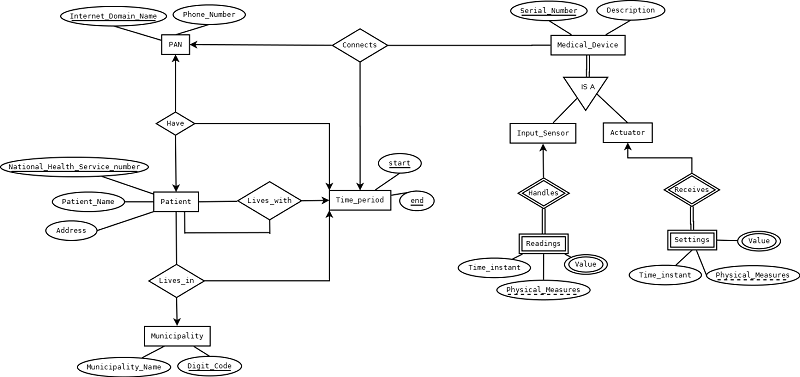
\includegraphics{Diagrama1.png}
\end{landscape}
\pagebreak

\section{Tabelas}
De acordo com o modelo E-R especificado anteriormente e com a metodologia estudada, a conversão em tabelas é feita da seguinte forma:

\begin{enumerate}
  \item Conversão de entidades fortes e suas especializações (quando aplicável):
  
  		\textit{Medical\_Device(\underline{Serial\_Number}, \underline{Manufacturer}, Description)}
  		
  		\textit{Input\_Sensor(\underline{Serial\_Number}, \underline{Manufacturer})}
  		
  			\tab{Serial\_Number:FK(Medical\_Device)}
  			
  			\tab{Manufacturer:FK(Medical\_Device)}
  			
  		\textit{Actuator(\underline{Serial\_Number}, \underline{Manufacturer})}
  		
  			\tab{Serial\_Number:FK(Medical\_Device)}
			
			\tab{Manufacturer:FK(Medical\_Device)}  
					
  		\textit{PAN (\underline{Internet\_Domain\_Name}, Phone\_Number)}
  		
  		\textit{Patient (\underline{National\_Health\_Service\_number}, Patient\_Name, Address, Internet\_Domain\_Name)}
  		
  				\tab{Internet\_Domain\_Name:FK(PAN)}
  				
  		\textit{Municipality (\underline{Digit\_code}, Municipality\_Name)}
  		
  		\textit{Time\_period (\underline{start}, \underline{end}, Internet\_Domain\_Name, National\_Health\_Service\_number)}
  		
  		\tab{Internet\_Domain\_Name:FK(PAN)}
  		
  		\tab{National\_Health\_Service\_number:FK(Patient)}
  		
  		\item Conversão de \textit{weak-entities}:
  		
  		\textit{Readings (\underline{Serial\_Number}, \underline{Manufacturer}, \underline{Physical\_Measures}, Value, Time\_instant)}
  			
  			\tab{Serial\_Number: FK(Input\_Sensor)}
  			
  			\tab{Manufacturer:FK(Input\_Sensor)}
  			
  		\textit{Settings (\underline{Serial\_Number}, \underline{Manufacturer}, \underline{Physical\_Measures}, Value, Time\_instant)}
  			
  			\tab{Serial\_Number: FK(Actuator)}
  			
  			\tab{Manufacturer:FK(Actuator)}
  			
  		\item conversão de relações:
  		
  		\textit{Connects (\underline{start}, \underline{end}, \underline{Serial\_Number},\underline{Manufacturer}, Internet\_Domain\_Name)}
  		
  		\tab{start: FK(Time\_period)}
  		
  		\tab{end: FK(Time\_period)}
  		
  		\tab{Serial\_Number: FK(Medical\_Device)}
  		
  		\tab{Manufacturer: FK(Medical\_Device)}
  		
  		\tab{Serial\_Number: FK(Actuator)}
  		
  		\tab{Internet\_Domain\_Name: FK(PAN)}
  		
  		\textit{Lives\_in (\underline{National\_Health\_Servive\_number, start, end}, Digit\_Code)}
  		
  		\tab{National\_Health\_Servive\_number:FK(Patient)}
  		
  		\tab{start: FK(Time\_period)}
  		
  		\tab{end: FK(Time\_period)}
  		
  		\tab{Digit\_Code: FK(Municipality)}
  		
  		\textit{Lives\_with(\underline{National\_Health\_Service\_number1, National\_Health\_Service\_number2, start, end})}
  		
  		\tab{National\_Health\_Service\_number1:FK(Patient)}
  		
  		\tab{National\_Health\_Service\_number2:FK(Patient)}
  		
  		\tab{start: FK(Time\_period)}
  		
  		\tab{end: FK(Time\_period)}  		
\end{enumerate}

De acordo com a metodologia, seguir-se-ia a conversão de agregações. Porém, por não atribuirmos nenhuma agregação não se construiu qualquer tabela para este conceito.
\end{document}